\chapter{几何光学与成像}
\label{ch:01}

\section{效果}
\label{sec:ch01-effect}

读完本章，你应能：
\begin{enumerate}
  \item 用针孔模型写出世界点 $(X,Y,Z)$ 到像面 $(u,v)$ 的投影关系，并说明其光学假设；
  \item 陈述薄透镜成像公式，分清焦距 $f$、物距 $s$、像距 $s'$，并能解释「对焦」在光路上做什么；
  \item 用弥散圆与景深相关量 $Z_d$ 解释：为何工作距一变，条纹或特征就糊；
  \item 区分理想投影与几何畸变，知道畸变为何必须进标定，而不是靠算法「硬抗」。
\end{enumerate}

\section{原理}
\label{sec:ch01-principle}

\subsection{针孔：投影几何的光学起点}

针孔相机假定：场景点与像点的连线穿过唯一光心，像成在光心后方的平面上。取光心为原点、光轴为 $Z$，则相似三角形给出
\begin{equation}
  u = f\frac{X}{Z},\qquad v = f\frac{Y}{Z},
  \label{eq:ch01-pinhole}
\end{equation}
其中 $f$ 为焦距（此处先理解为「光心到像面距离」的几何量）。齐次形式与内参矩阵写法留给 \chapref{ch:02}；本章先抓住光学含义：\textbf{直线光线、单一光心、像面垂直光轴}。

\begin{figure}[htbp]
  \centering
  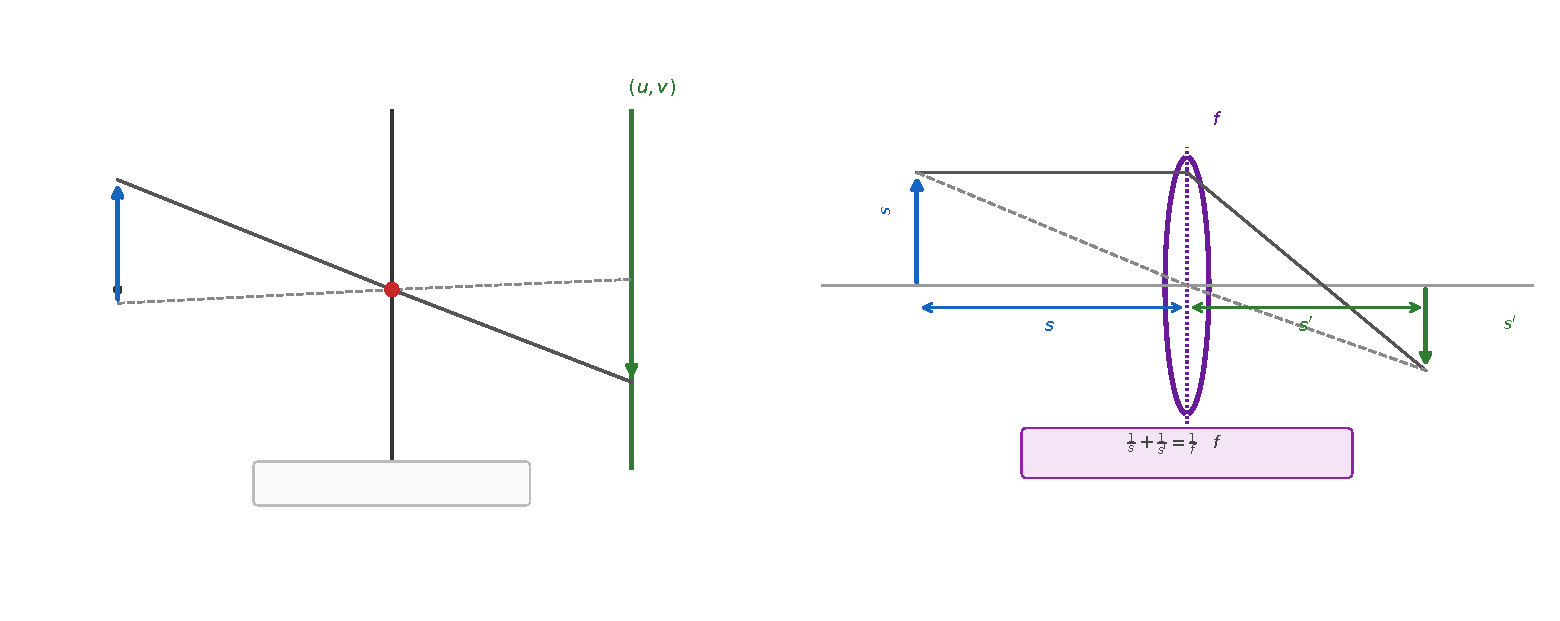
\includegraphics[width=0.95\textwidth]{fig-pinhole-thinlens.pdf}
  \caption{针孔与薄透镜成像概念草图（非精确工程图）。左：光线过针孔，像倒立。右：薄透镜把物距 $s$、像距 $s'$ 与焦距 $f$ 联系起来。}
  \label{fig:ch01-pinhole-thinlens}
\end{figure}

针孔模型\textbf{没有}「对焦」自由度：孔径理想化为点，几何上处处清晰。真实镜头有限孔径，必须引入透镜与离焦——否则无法讨论景深，而这正是近距离医学重建的痛点。

\subsection{薄透镜：对焦与放大率}

旁轴、单色、薄透镜假设下，物距 $s$、像距 $s'$、焦距 $f$ 满足
\begin{equation}
  \frac{1}{s}+\frac{1}{s'}=\frac{1}{f}.
  \label{eq:ch01-thinlens}
\end{equation}
约定：$s,s',f$ 取合适符号约定下的正值讨论（实物、实像、会聚透镜的常见课设约定）；工程实现以厂商与标定文档为准。横向放大率
\[
  m = -\frac{s'}{s}
\]
说明像倒立（负号）且大小由共轭距决定。

\textbf{对焦}在操作上常表现为调节 $s'$（传感器相对镜头的轴向位置）或等效地改变光学组，使给定工作距 $s$ 满足式~\eqref{eq:ch01-thinlens}。对焦不准时，点光源在像面张成弥散斑，而不是式~\eqref{eq:ch01-pinhole} 里的理想点。

有效焦距还会随波长 $\wavelength$ 略变（色散），导致不同颜色的对焦面分离——色差；本章先记一笔，系统展开见 \chapref{ch:08}。折射率 $n$ 进入透镜制造商公式，本书够用层面只需知道：$f$ 由曲率与 $n$ 决定，浸液或窗口玻璃会改共轭关系。

\subsection{有限孔径、弥散圆与景深}

设对焦在物距 $s$，传感器在对应的 $s'$。若物点改到 $s+\Delta s$，理想像面移离传感器，光束在传感器上截出直径为 $c$ 的\textbf{弥散圆}（circle of confusion）。当 $c$ 小于判据 $c_{\max}$（由像素尺寸或可容忍模糊决定）时，该物距仍被视为「可接受清晰」。前后可接受的物距范围，构成景深；文中用 $Z_d$ 统称与景深相关的特征尺度（如景深总长、前/后景深），\textbf{勿}与世界坐标 $Z$ 混用而不加下标。

定性规律（旁轴、常见摄影/机器视觉直觉，精确公式依光圈与放大率而定）：
\begin{itemize}
  \item 容许弥散圆 $c_{\max}$ 越大，表观景深越大；
  \item 相对孔径越大（光圈越大）、焦距 $f$ 越长、放大率越高，景深越窄；
  \item 近距离大放大率（口内、显微）时 $Z_d$ 往往只有毫米量级，牙面起伏即可离焦。
\end{itemize}

\begin{figure}[htbp]
  \centering
  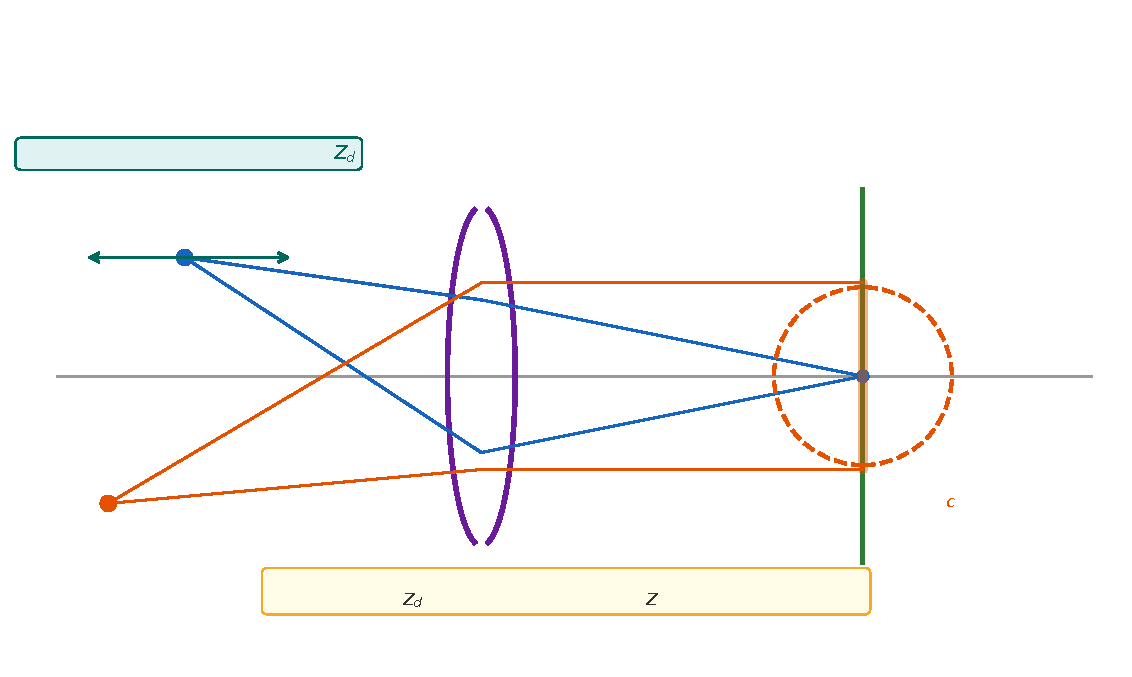
\includegraphics[width=0.92\textwidth]{fig-dof-coc.pdf}
  \caption{景深与弥散圆概念草图。对焦物点在像面收为清晰点；离焦物点张成弥散圆。可接受的物距范围与 $Z_d$ 相关。}
  \label{fig:ch01-dof}
\end{figure}

数值孔径 $\NA$ 在显微与浸液物镜中更常用；与 $f$ 数相关：$F\# \approx 1/(2\NA)$（空气、小角度近似）。$\NA$ 越大，分辨本领往往越好，但景深越窄——分辨率与 $Z_d$ 的折中在 \chapref{ch:03}、\chapref{ch:08} 还会出现。

\subsection{几何畸变：直线不再直}

理想针孔把空间直线投成直线。实际镜头的径向畸变等使像点沿径向伸缩：桶形（中间放大相对小）或枕形（相反）。切向畸变与装配偏心有关。畸变是\textbf{像面坐标的非线性映射}，不能靠提高 $\SNR$ 消除；必须在投影模型中参数化并标定（\chapref{ch:02}）。

对结构光而言：若解码假设「投影行/列对应直线栅」，而相机侧畸变未校正，相位到 $(X,Y,Z)$ 的映射会出现系统性弯曲——点云里牙弓被「掰弯」，常被误诊为算法 bug。

\subsection{从几何光学到计算机视觉投影}

机器视觉把式~\eqref{eq:ch01-pinhole} 像素化：$f$ 以像素计，并加入主点 $(c_x,c_y)$，写成内参 $K$。光学上，$f$ 仍源于像距与透镜；主点接近光轴与传感器交点。外参 $R,t$ 把世界系变到相机系，本身不是光学元件参数，但与标定板姿态、手持扫描轨迹耦合。\citet{HartleyZisserman2004} 给出多视几何全貌；本章要求先建立「$f$、对焦、$Z_d$、畸变」的光学直觉，再进入 \chapref{ch:02} 的矩阵与可观性。


\subsection{物像共轭与「清晰」的操作定义}

工程上说一张图「清晰」，通常指点状特征的能量落在可接受的弥散圆内，而不是数学上的狄拉克点。对结构光，还要在\textbf{条纹空间频带}内保持足够调制度：即使主观看「还行」，高频条纹的对比度仍可能先塌掉。因此同一光圈下，摄影可接受的 $Z_d$ 可以宽于相位测量可接受的 $Z_d$。写设计文档时建议显式给出：
\begin{itemize}
  \item 判据 $c_{\max}$（例如 $1$--$2$ 像素，或与相位误差上限反推）；
  \item 对应的工作距区间与允许探头倾角；
  \item 在该区间内条纹对比度的下限（实测）。
\end{itemize}

\subsection{窗口、浸液与物距的「表观」变化}

保护玻璃、唾液膜或空气–介质界面会使光线折射，等效物距与主面位置偏移。薄透镜公式仍可作\textit{一阶}直觉，但标定得到的有效 $f_x$ 已吸收部分窗口效应；若标定在空气中完成、扫描在另一介质窗口下进行，等于更换了光路却未更换 $K$。医学近距设备务必保证\textbf{标定光路与工作光路一致}（含窗口），否则 \chapref{ch:02} 的可观性讨论会建立在错误的物理上。

\subsection{推导：弥散圆直径与景深公式}

前面给出的是定性规律，这里把它推成可以算数的公式，并写清楚每一步的近似。

\textbf{第一步：轴向放大率。} 对薄透镜式~\eqref{eq:ch01-thinlens} 两边求微分：$-\mathrm{d}s/s^2-\mathrm{d}s'/s'^2=0$，故
\[
  \Delta s'\approx-\frac{s'^2}{s^2}\,\Delta s=-m^2\,\Delta s .
\]
物点沿轴移动 $\Delta s$，像点反向移动 $m^2$ 倍。近距、放大率接近 $1$ 时轴向与横向放大同量级；放大率小（远景）时像点几乎不动，这就是远景景深大的根源。条件：$|\Delta s|\ll s$，一阶展开成立。

\textbf{第二步：相似三角形。} 设入瞳直径 $D=f/N_F$（$N_F$ 为工作 F 数）。会聚到 $s'+\Delta s'$ 的光锥在传感器（位于 $s'$）上截出的圆直径为
\[
  c\approx D\,\frac{|\Delta s'|}{s'}=\frac{f}{N_F}\,\frac{m^2|\Delta s|}{s'} .
\]
条件：$|\Delta s'|\ll s'$，且忽略衍射（第~\ref{ch:03}~章再补）。

\textbf{第三步：反解景深。} 令 $c=c_{\max}$，前后对称近似下总景深
\[
  Z_d\approx 2|\Delta s|_{\max}=\frac{2c_{\max}N_F\,s'}{f\,m^2}.
\]
再用 $s'=f(1+|m|)$（由式~\eqref{eq:ch01-thinlens} 与 $|m|=s'/s$ 得到），最终
\begin{equation}
  Z_d\approx\frac{2\,c_{\max}\,N_F\,(1+|m|)}{m^{2}} .
  \label{eq:ch01-dof}
\end{equation}
这是近摄与机器视觉中常用的景深式。它把定性规律量化了：$Z_d$ 与 $N_F$、$c_{\max}$ 成正比，与 $m^2$ 近似成反比。适用条件：薄透镜、旁轴、$|\Delta s|\ll s$、入瞳与出瞳大小相近（瞳放大率接近 $1$）。远景（$|m|\to0$ 且物距接近超焦距）时前后景深不再对称，此式不适用。

\textbf{例（数量级示意）。} 口内相机看 $15\,\mathrm{mm}$ 宽的视场，传感器宽 $6\,\mathrm{mm}$，故 $|m|=0.4$。像元 $3\,\mu\mathrm{m}$，取 $c_{\max}=2$ 像素 $=6\,\mu\mathrm{m}$。
\begin{itemize}
  \item $N_F=8$：$Z_d\approx2\times0.006\times8\times1.4/0.16\approx0.84\,\mathrm{mm}$；
  \item $N_F=16$：$Z_d\approx1.7\,\mathrm{mm}$。
\end{itemize}
单颗牙的起伏就有数毫米，按「两像素弥散」的判据，几何景深远远不够。这个例子引出两个要在后文回答的问题：其一，缩小光圈换景深会被衍射限制住（像方艾里斑直径约 $2.44\,\lambda N_F(1+|m|)$，$\lambda=450\,\mathrm{nm}$、$N_F=8$ 时约 $12\,\mu\mathrm{m}$，已超过 $c_{\max}$，见第~\ref{ch:03}~章）；其二，结构光并不要求「点」清晰，只要求条纹调制度不塌。对称的模糊只降低正弦条纹的幅度、不移动其相位，所以条纹解码能容忍比角点检测大得多的弥散圆（第~\ref{ch:08}~章用 $\MTF$ 量化）。

\subsection{推导：平板窗口引起的焦点偏移}

口内探头前端常有保护窗或反射镜，显微与内窥中还有盖玻片和浸液。厚度 $t$、折射率 $n$ 的平行平板插在会聚光路中，旁轴近似下会把像点沿轴推远
\[
  \Delta=t\Bigl(1-\frac{1}{n}\Bigr).
\]
推导：光线在平板内折射，入射角 $\theta$ 与折射角 $\theta'$ 满足 $\sin\theta=n\sin\theta'$；穿过平板的横向偏移使光线延长线与轴的交点后移 $t(1-\tan\theta'/\tan\theta)$，旁轴时 $\tan\theta'/\tan\theta\approx1/n$。条件：小角度；大 $\NA$ 时不同孔径带的偏移不同，出现球差。

例：$t=2\,\mathrm{mm}$、$n=1.5$，$\Delta\approx0.67\,\mathrm{mm}$。若标定时没装窗口、扫描时装上，或换了不同厚度的窗口，对焦面与标定内参都会变。这比上面算出的景深还要大，不能忽略。

\section{限度}
\label{sec:ch01-limits}

\begin{itemize}
  \item 旁轴与薄透镜忽略厚透镜主面、场曲、像散等；广角或大视场口内镜头常需更完整模型。
  \item 针孔无衍射：分辨率下限由波动光学给出，$\PSF$/$h$ 与 $\MTF$ 见后续章。
  \item 景深判据 $c_{\max}$ 依赖任务：亚像素相位对模糊比「看看清」更严，故结构光有效 $Z_d$ 往往短于摄影学宣传值。
  \item 畸变模型是近似；极强畸变或非中心投影镜头可能需鱼眼或其他参数化。
\end{itemize}

\section{对象}
\label{sec:ch01-object}

\textbf{场景 A：口内结构光工作距。} 声称景深 $Z_d\approx 10\,\mathrm{mm}$，实际牙尖到沟底高差可达数毫米且探头倾斜。若对焦面设在牙尖，沟底条纹对比度崩溃——点云「顶清底糊」。处置：缩小光圈（换 $\SNR$）、分层对焦融合、或限制姿态使工作距落在 $Z_d$ 内。

\textbf{场景 B：标定板拍得「很锐」但重建弯。} 锐利只说明对焦好；未建模的桶形畸变仍使棋盘格直线弯曲，估出的 $K$ 与射线方向错，三角测量系统性偏。处置：在模型中加径向/切向项并看重投影误差是否各向同性下降。

\textbf{场景 C：把摄影 $f$ 数当算法超参乱调。} 开大光圈提亮却吃掉 $Z_d$；在 CUDA 里加大双边滤波，不如先固定光圈与曝光做光学预算。灰度亮不代表 $E$ 与 $\SNR$ 在条纹频带内够用。


\section*{本章收束}
针孔给出投影骨架，薄透镜给出对焦与 $f$，弥散圆给出 $Z_d$，畸变逼你改模型。把这些写进口内/近距结构光的检查清单后，才能在下一章进入 $K$、畸变参数与标定可观性，而不把矩阵当成纯代数游戏。

\section{习题}
\label{sec:ch01-exercises}

\begin{enumerate}
  \item \textbf{（概念）} 针孔模型为何无法解释「对焦旋钮」？薄透镜模型如何补上？
  \item \textbf{（计算）} 设 $f=12\,\mathrm{mm}$，物距 $s=40\,\mathrm{mm}$。求像距 $s'$。若传感器固定在该 $s'$，物距改为 $45\,\mathrm{mm}$，定性说明像面弥散变大还是变小（不必精确 $c$）。
  \item \textbf{（计算）} 世界点 $(X,Y,Z)=(5,0,100)\,\mathrm{mm}$，针孔 $f=8\,\mathrm{mm}$（单位一致）。求理想像点 $(u,v)$（光心原点、主点在原点）。
  \item \textbf{（重建场景）} 近距扫描中缩小光圈后条纹更「到处都能看清」，但噪声明显变大。用 $Z_d$ 与 $\SNR$ 解释权衡，并给出一条可执行的折中策略。
  \item \textbf{（概念）} 为何说畸变导致的点云弯曲通常不能靠提高曝光消除？
  \item \textbf{（诊断）} 棋盘格照片四角发糊、中心锐：更可能是场曲/像面不理想，还是单纯整体离焦？对标定姿态选择有何启示？
  \item \textbf{（符号）} 文中 $Z_d$ 与深度 $Z$ 同时出现时如何避免混淆？举例写一句正确表述。
  \item \textbf{（推导）} 从式~\eqref{eq:ch01-thinlens} 出发，独立推出轴向放大率 $\Delta s'\approx-m^2\Delta s$，并说明 $|m|=1$ 时它的物理含义。
  \item \textbf{（计算）} 用式~\eqref{eq:ch01-dof}，$|m|=0.2$、$N_F=8$、$c_{\max}=6\,\mu\mathrm{m}$，求 $Z_d$。与正文 $|m|=0.4$ 的结果相比，放大率减半景深变为几倍？代价是什么？
  \item \textbf{（计算）} 正文例中，若要求像方艾里斑直径不超过 $c_{\max}=6\,\mu\mathrm{m}$（$\lambda=450\,\mathrm{nm}$，$|m|=0.4$），$N_F$ 最大取多少？此时几何景深是多少？
  \item \textbf{（口扫场景）} 探头前窗由 $1.0\,\mathrm{mm}$ 换为 $2.0\,\mathrm{mm}$（同为 $n=1.5$），焦点偏移变化多少？给出必须重新做的两件事。
  \item \textbf{（C++/CUDA 实践）} 写出一个函数的接口与内部步骤：输入 $f$、$N_F$、$s$、像元间距与 $c_{\max}$（以像素计），输出前后景深。指出哪一步需要检查适用条件并返回错误。
\end{enumerate}

\section{习题讲解}
\label{sec:ch01-solutions}

\begin{enumerate}
  \item 针孔孔径为零、几何上处处清晰，没有共轭面可调。薄透镜有式~\eqref{eq:ch01-thinlens}，调节 $s'$（或等效）使给定 $s$ 成像在传感器上，即对焦。
  \item $\frac{1}{s'}=\frac{1}{f}-\frac{1}{s}=\frac{1}{12}-\frac{1}{40}=\frac{10-3}{120}=\frac{7}{120}$，故 $s'=\frac{120}{7}\approx17.14\,\mathrm{mm}$。物距变到 $45\,\mathrm{mm}$ 时理想 $s'$ 变小，传感器仍在原处 → 离焦，弥散圆变大。
  \item $u=fX/Z=8\times5/100=0.4\,\mathrm{mm}$，$v=0$。
  \item 小光圈增大 $Z_d$（更处处可接受清晰），但进光少，$\SNR$ 下降，相位/匹配方差升。折中：固定可接受 $Z_d$ 的最大光圈，用曝光时间或增益补 $\SNR$，并防运动模糊；或多曝光融合。
  \item 畸变是几何映射，不随光子数增加而线性校正；曝光主要改 $\SNR$ 与饱和，不改径向多项式形状。
  \item 更像场曲或像差随视场变化，而非单一全局离焦（全局离焦中心也会糊）。标定应覆盖实际工作视场，并检查角点重投影误差是否随半径增大。
  \item 例：「工作距落在景深特征量 $Z_d$ 内时，世界坐标深度 $Z$ 上的点云方差下降。」出现景深时用 $Z_d$，场景深度用 $Z$ 或 $(X,Y,Z)$。
  \item 微分 $1/s+1/s'=1/f$：$-\mathrm{d}s/s^2-\mathrm{d}s'/s'^2=0$，故 $\mathrm{d}s'=-(s'/s)^2\mathrm{d}s=-m^2\mathrm{d}s$。$|m|=1$ 时物点移动多少、像点就反向移动多少，对应 $s=s'=2f$ 的一倍成像。
  \item $Z_d\approx2\times0.006\times8\times1.2/0.04\approx2.9\,\mathrm{mm}$，约为 $|m|=0.4$ 时 $0.84\,\mathrm{mm}$ 的 $3.4$ 倍（$(1+|m|)/m^2$ 之比 $30/8.75$）。代价：同样传感器视场变大、物方每像素对应更大尺寸，$f_x$ 对应的物方分辨率下降，同样 $\delta d$ 带来的横向误差变大。
  \item $2.44\times0.45\,\mu\mathrm{m}\times N_F\times1.4\le6\,\mu\mathrm{m}$，得 $N_F\le3.9$，取 $N_F\approx4$。此时 $Z_d\approx2\times0.006\times4\times1.4/0.16\approx0.42\,\mathrm{mm}$。在这个放大率和像素下，「几何清晰」与「衍射清晰」同时满足时景深只有约 $0.4\,\mathrm{mm}$，说明必须放宽判据（依靠条纹对模糊的容忍）而不是一味缩光圈。
  \item 偏移由 $0.33\,\mathrm{mm}$ 变为 $0.67\,\mathrm{mm}$，变化约 $0.33\,\mathrm{mm}$，与景深同量级。必须：重新对焦（或确认对焦面仍覆盖工作距）；在新窗口下重新标定内参与畸变（大 $\NA$ 时窗口还引入球差）。
  \item 接口：输入 \texttt{f\_mm}、\texttt{NF}、\texttt{s\_mm}、\texttt{p\_mm}、\texttt{cmax\_px}，输出 \texttt{near\_mm}、\texttt{far\_mm}。步骤：(1) $s'=fs/(s-f)$，检查 $s>f$；(2) $|m|=s'/s$；(3) $c_{\max}=c_{\max,\mathrm{px}}\cdot p$；(4) $|\Delta s|=c_{\max}N_Fs'/(fm^2)$；(5) 检查 $|\Delta s|\ll s$（如小于 $0.1s$），否则返回「一阶近似失效」或改用精确前后景深公式。单位全部用毫米，像素只在输入处换算一次。
\end{enumerate}
